\clearpage
\section{Background estimation for processes with genuine \texorpdfstring{\met}{MET}\label{sec:backgrounds}}

After applying the full hadronic selection, the remaining 
backgrounds are SM processes with genuine \met in the final state. 
In the category of zero b-tagged jets, the two primary background sources are:
\begin{itemize}
\item \zj; where the Z boson decays into a pair of neutrinos, 
\item \wj; where the W boson either undergoes a leptonic decay 
and the lepton is lost or it undergoes the weak decay $\wtaunu$ where the $\tau$ decays into quarks
\end{itemize}
%
%a ``lost'' lepton is defined as any lepton that isn't reconstructed or 
%fails the isolation or acceptance requirements. 
Other SM backgrounds, such as the diboson production ($WW,\,ZZ,\,WZ$), single-top, and 
Drell-Yan ($Z/\gamma^{*} \ra l\bar{l}$) are also expected, but at lower yields.

For events with one or more b-tagged jets, the decay of \ttbar, where each
top decays into a b-quark and a W boson which in turn decays into 
a lost lepton and a neutrino, also becomes a large background source.
For events with two reconstructed b-quark jets, \wj and \zj are suppressed
and \ttbar production dominates the background. 

This analysis uses a ``data-driven'' method to estimate backgrounds
in the hadronic search region. Data control samples are used to predict
the SM background yields instead of estimating them from MC simulations. 
This approach has two benefits. First, the beam and detector conditions 
for the hadronic and control data samples are very similar, therefore there 
is no need to rely on MC simulation getting the detector conditions correct,
which is difficult. Second, the information used from MC simulation is largely in the form of 
ratios (Section~\ref{sec:background-method}), which has the benefit of canceling 
potential systematic effects or biases from the simulation.

Two different control samples are used to estimate the backgrounds. To estimate the
\znunu + jets background, $\gamma$ + jets events are utilzed. They have the same
kinematic properties as \znunu + jets when the photon is ignored, but 
different acceptance~\cite{PAS-SUS-08-002,Bern:2011pa}. A \mj control
sample is used to estimate all remaining backgrounds including the 
dominant \wj and \ttbar process.
%The final results are obtained through a maximum likelihood fit described
%in chapter~\ref{sec:statistics}. 
The following sections describe the estimation method and control samples used 
for the estimation.

\subsection{Overview of the method\label{sec:background-method}}

For a given bin in \scalht, \njet, \nb, the method predict the number 
of events expected from background processes in the hadronic search region ($\npre^{\rm  had}$) 
by translating from the observed data yield in a control region 
($\nobs^{\rm  control}$) through the use of a {\it translation factor} 
(TF) constructed from the ratio of MC hadronic and control yields, ie:
\begin{equation}
  \label{equ:pred-method}
  \npre^{\rm had} = \underbrace{\frac{N_{\rm MC}^{\rm
      had}}{N_{\rm MC}^{\rm
      control}}}_\text{translation factor}\! \times \; \nobs^{\rm    control},   
\end{equation}
%In the final fit, the expected yield is used rather than the observed yield
%$\nobs^{\rm  control}$, nonetheless the observed yield is used here for 
%illustration.
where $N_{\rm MC}^{\rm had}$ is the number of expected events of the background
source(s) in the hadronic selection that are present in the control region under study.
$N_{\rm MC}^{\rm control}$ is the sum of expected yields from all MC samples, 
obtained for the relevant control sample selection:
\begin{equation}
  \label{equ:ratio-denom}
  N_{\rm MC}^{\rm control} = N_{\rm W} + N_{\ttbar} + N_{\znunu} +
N_{\rm DY} + N_{\gamma} + N_{\rm top} + N_{\rm di-boson}
\end{equation}
Depending on the b-tag category, one or both control samples are used 
to predict the backgrounds in the hadronic search region. For the b-jet 
multiplicity bins $n_b = 0$ and $n_b = 1$, the \mj and \gj control samples 
are used to predict the total background. The \gj control
sample is used to predict the \znunu + jets background and the expected yield
obtained from the \znunu sample enters the numerator of each translation
factor:

\begin{equation}
  \label{equ:ratio-numer-gj}
  N_{\rm MC}^{\rm had}(\scalht,\njet,\nb \leq 1) = N_{\znunu}.
\end{equation}
%
For the same b-tag categories, the \mj control sample is used to predict 
the remaining SM background processes, namely the W + jets, \ttbar + jets,
Drell-Yan, di-boson and single top backgrounds, and the total expected yield
from these processes enter the numerator of each translation factor:
%
\begin{equation}
  \label{equ:ratio-numer-mj}
  N_{\rm MC}^{\rm had}(\scalht,\njet,\nb \leq 1) = N_{\rm W} +
  N_{\ttbar} + N_{\rm DY} + N_{\rm top} + N_{\rm di-boson}
\end{equation}

Only the \mj control sample is used to predict the background in the 
the b-tag multiplicity bin $n_b = 2$. The \gj control sample is not 
used as the yield in this data control sample is expected to be low
due to the requirement of at least two b-jets per event. The method of
using a W + jets sample to predict the \znunu\ + jets background has
been used previously~\cite{RA1Paper, RA1Paper2011, RA1Paper2012}.  
Therefore the total predicted expected yield from all processes 
enter the numerator of each translation factor:
%
\begin{equation}
  \label{equ:ratio-numer-mj-tot}
  N_{\rm MC}^{\rm had}(\scalht,\njet,\nb = 2) = N_{\rm W} +
  N_{\ttbar} + N_{\rm DY} + N_{\rm top} + N_{\rm di-boson} + N_{\znunu}
\end{equation}
%
\indent The control samples used to predict the SM backgrounds for each 
event category are summarized in Table~\ref{tab:fit-plots}.
A detailed example of the background estimation procedure is given
in Appendix~\ref{app:bkg-example}. 
Tables~\ref{tab:results-PHOTON_0b_le3j}--\ref{tab:results-W_2b_ge4j}
in Appendix~\ref{app:bk-yields} show the control sample yields, translation
factors, hadronic MC yields, for each control sample in each category.
%\input{figures/tables/v22/background/tables_0b_le3j.tex}
The control sample selections are described in the following
sections. 
%
\begin{table}[ht!]
  \caption{Summary of control samples used to predict the SM
    background for each event category. }
  \label{tab:fit-plots}
  \centering
  \begin{tabular}{ lll }
    \hline
    \hline
    \njet   & \nb     & Control samples \\ [1.0ex]
    \hline
    2--3    & 0       & \mj,  \gj  \\
    2--3    & 1       & \mj,  \gj  \\
    2--3    & 2       & \mj        \\
    $\geq$4 & 0       & \mj,  \gj  \\
    $\geq$4 & 1       & \mj,  \gj  \\
    $\geq$4 & 2       & \mj             \\
    \hline
    \hline
  \end{tabular}
\end{table}


%The selection criteria for the three control samples closely resemble
%those for the signal region, differing mainly through the use of a
%muon, di-muon, or photon {\it tag} (that is ignored in the calculation
%of jet-based kinematic variables such as \scalht, \mht, \alphat, \etc)
%and some minimal additional kinematic requirements (\eg invariant or
%transerve mass windows) to obtain W, Z, and \ttbar-enriched event
%samples. The same selection criteria are designed to suppress signal
%contamination in the control samples so that unbiased data-driven
%estimates for the SM backgrounds in the signal region can be
%made. Hence, we refer to these samples as {\it control} samples
%although in the final simultaneous fit, any potential signal
%contamination is properly taken into account.
%
%The control sample definitions and binning scheme are chosen so that
%the reliance on simulation to extrapolate correctly from a control
%region to the signal region is minimised. Many systematic effects are
%expected to cancel largely in the translation factor. However, a
%systematic uncertainty is assigned to each translation factor to account
%for theoretical uncertainties and effects such as the mismodelling of
%kinematics (\eg acceptances) and instrumental effects (\eg
%reconstruction efficiencies), as described in
%Sec.~\ref{sec:bkgd-syst}.
%
%%Kinematic cuts are applied to enrich as much as possible the \wj,
%%\ttbar, and \znunu components in the muon and di-muon control
%%samples. The definition of the samples are geared towards efficiency
%%rather than purity (even so, the purities are at the level $>$90\%)
%%and any contamination from "backgrounds" (\eg \ttbar in the case of
%%the \mmj sample) are simply incorporated into the translation
%%factors. Alternatively, a zero b-jet requirement can be applied to the
%%\mmj sample to obtain a higher purity of Z$\rightarrow\mu\mu$ + jets
%%events (\ie, with reduced contamination from \ttbar), which can then
%%be used to give an expectation for the \znunu + jets background for
%%all b-jet categories in the signal region.
%
\subsection{Definition of the control samples\label{sec:def-control-samples}}

\subsubsection{Muon and photon triggers\label{sec:muon_triggers}}

Events for the muon control sample are recorded with the \verb!HLT_IsoMu24_eta2p1! 
trigger. Figure~\ref{fig:eff-muon} (left) shows the \verb!HLT_IsoMu24_eta2p1! 
trigger efficiency as determined in bins of number of primary vertices 
for muon $\pt >$ 25 \gev and $|\eta| <$ 2.1~\cite{ref:muon-eff}.
Figure~\ref{fig:eff-muon} (right) shows the distribution of the number 
of vertices in the muon control sample seeded by the \verb!HLT_IsoMu24_eta2p1!. 
The efficiency at the mean number of vertices $n_{vtx}=13$ is taken as flat
trigger efficiency across \njet, \nb, and \scalht. This measurement 
agrees well with direct tag and probe measurements in bins of 
\njet, \nb, \scalht done elsewhere~\cite{RA1Paper2012}.

\begin{figure}[!h]
  \begin{center}
  \subfigure{
    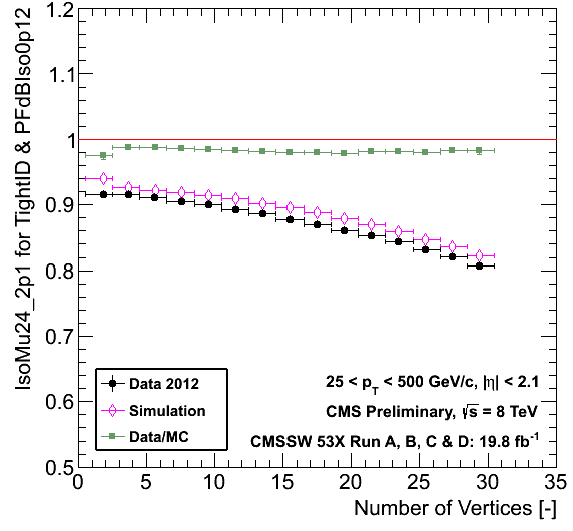
\includegraphics[width=0.3\textwidth,]{figures/trigger/muonEffvsNvtx}
    }   
  \subfigure{
   \includegraphics[width=0.42\textwidth,page=65]{figures/data-mc/v21/mu/muonLook_pfJet_ge2j_375.pdf}
   }\\     
    \caption{\label{fig:eff-muon}
    (left) Muon trigger efficiency as a function of
    number of primary vertices for muon $\pt>$ 25 \gev and
    $|\eta| <$ 2.1. (right) Number of primary vertices
    in muon control sample.} 
 
  \end{center}
\end{figure}

Events for the photon control sample are recorded with the
\verb!HLT_Photon150! trigger, which is $\sim100\%$ efficient for
$E_{\rm T}^{\rm photon} > 165\gev$ and $\scalht > 375\gev$, as shown
in Figure~\ref{fig:eff-photon}. The efficiency measurement is made
using the \verb!HLT_Photon90! trigger as a reference.

\begin{figure}[!h]
  \begin{center}
  \subfigure[\njetlow]{
    \includegraphics[width=0.43\textwidth,page=6]{figures/trigger/g_barrel_375_caloJet_le3j_}
    }   
  \subfigure[\njethigh]{
   \includegraphics[width=0.43\textwidth,page=6]{figures/trigger/g_barrel_375_caloJet_ge4j_}
   }\\     
    \caption{\label{fig:eff-photon}
    Cumulative efficiency turn-on curves for the \texttt{HLT\_Photon150} trigger 
    as a function of photon \pt for events satisfying \njetlow 
    (left) and \njethigh (right).} 
  \end{center}
\end{figure}

\FloatBarrier


\subsubsection{The \texorpdfstring{\mj}{muon plus jets} control sample\label{sec:muonSelection}}

\wj and \ttbar processes are found in the hadronic search region 
when the decay lepton is missed by the lepton veto, either 
because it was not reconstructed properly, fell out of acceptance 
or alternatively, decayed hadronically in the case of a tau lepton 
from a high-p$_{T}$ W boson. Instead of directly relying on MC 
simulation to estimate these backgrounds, a \mj control sample is 
used where the selection criteria is chosen to identify W bosons 
decaying to a muon and a neutrino. Then, by removing the muon from 
the event, one effectively selects a sample of W boson decaying to 
a neutrino and a lost lepton. In order to select events containing 
W bosons, exactly one tight isolated muon~\ref{sec:reconstruction} 
with of \PT $>$ 30 \gev and $|\eta| <$ 2.1 is required, 
and the transverse mass of the W candidate, 
$M_{T} = \sqrt{2\pt^{\mu}\met(1-cos(\Delta\phi(\vec{p}^{\rm  \mu},\met))}$ 
must be between 30 and 125~\gev.  Events are vetoed if a muon is found inside
a jet, i.e. $\Delta R(\mu,\textrm{jet}) < 0.5$. The single isolated track 
veto, described in Sections~\ref{sec:recSIT} and~\ref{sec:vetoes}, is applied. 
The veto considers all single isolated tracks in the event except 
that associated with the identified, isolated muon. The cleaning cut 
$\mht/\pfmet$ described in ~\ref{sec:finalSelections} is also applied, 
where the \pfmet is adjusted to exclude the muon's transverse momentum.
This modification ensures that the quantities \mht and \pfmet can be 
compared. Lastly, while all other jet-based quantities, like \scalht 
and \mht, are kept consistent with those applied in the hadronic 
search region, the \alphat requirement is removed. This modification 
increases the statistical power of the sample. Removing the \alphat 
requirement is only made possible by the control sample's kinematic 
cuts which ensure the selection of electroweak processes while keeping
contamination from multijet QCD events negligible. Because the control 
sample is used to extrapolate yields in a hadronic search region, 
which includes the \alphat requirement, a closure test as been devised 
and explained in Section~\ref{sec:closure-tests-desc} to demonstrate that no 
significant biases are seen from the exclusion of the \alphat cut. Comparisons
of data and simulated SM processes key variables relevant to 
the muon control sample are shown in Figure~\ref{fig:control-plots-muon}. 

\begin{figure}[h!]
  \centering
  \subfigure[muon \pt distribution ($\njet \geq 2$, $\nb \geq 0$).]{
    \label{fig:figures_pt_all}
    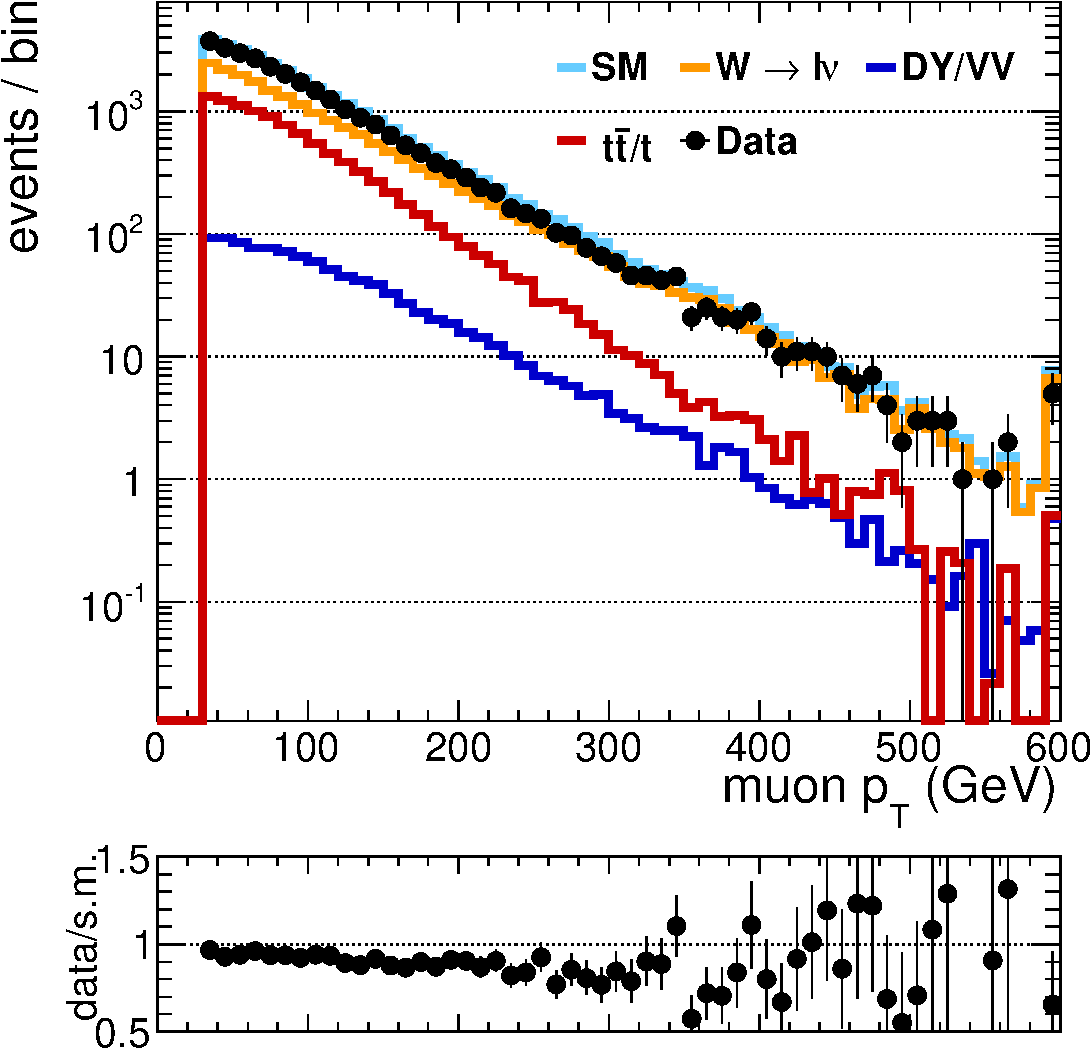
\includegraphics[width=0.4\textwidth]{figures/data-mc/v22/mu/muonLook_pfJet_ge2j_375_pt.pdf}
  } 
  \subfigure[muon $\eta$ distribution ($\njet \geq 2$, $\nb \geq 0$)]{
    \label{fig:figures_eta_all}
    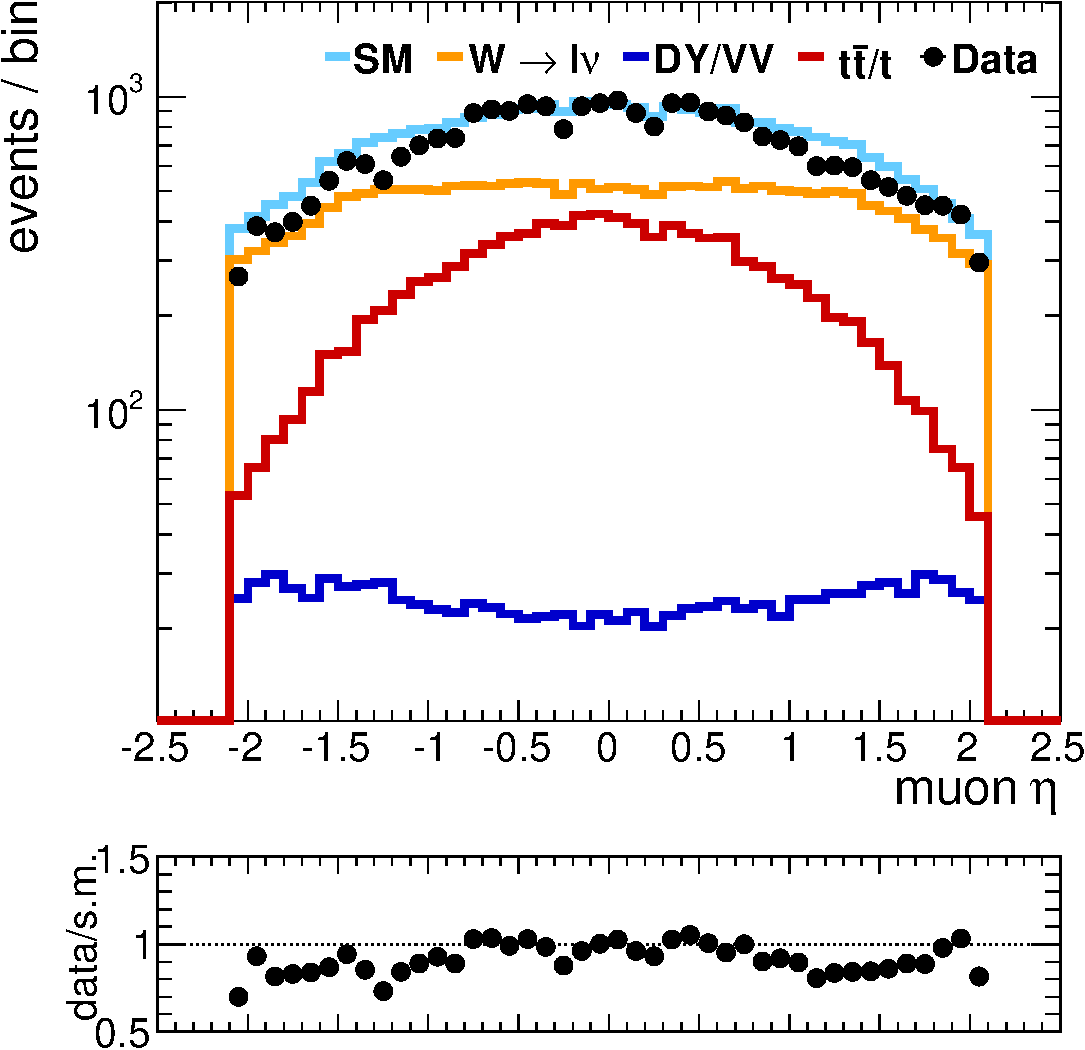
\includegraphics[width=0.4\textwidth]{figures/data-mc/v22/mu/muonLook_pfJet_ge2j_375_eta.pdf}
  } \\
  \subfigure[\nb distribution ($\njet \geq 2$, $\nb \geq 0$)]{
    \label{fig:figures_nb_1}
    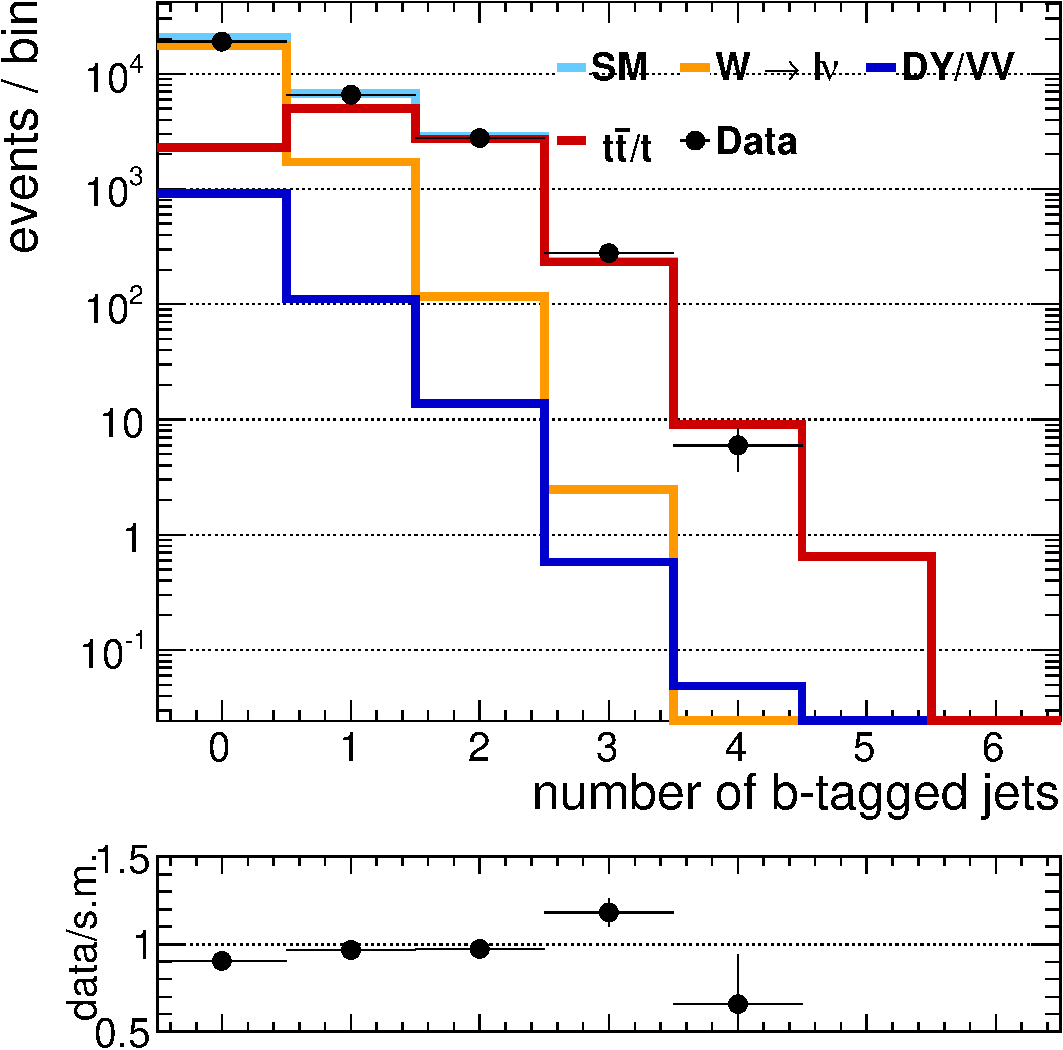
\includegraphics[width=0.4\textwidth]{figures/data-mc/v22/mu/muonLook_pfJet_ge2j_375_xcak5JetPFIndicesBtagged2Pat.pdf}
  } 
  \subfigure[\scalht distribution ($\njet \geq 2$, $\nb \geq 0$)]{
    \label{fig:figures_HT_0}
    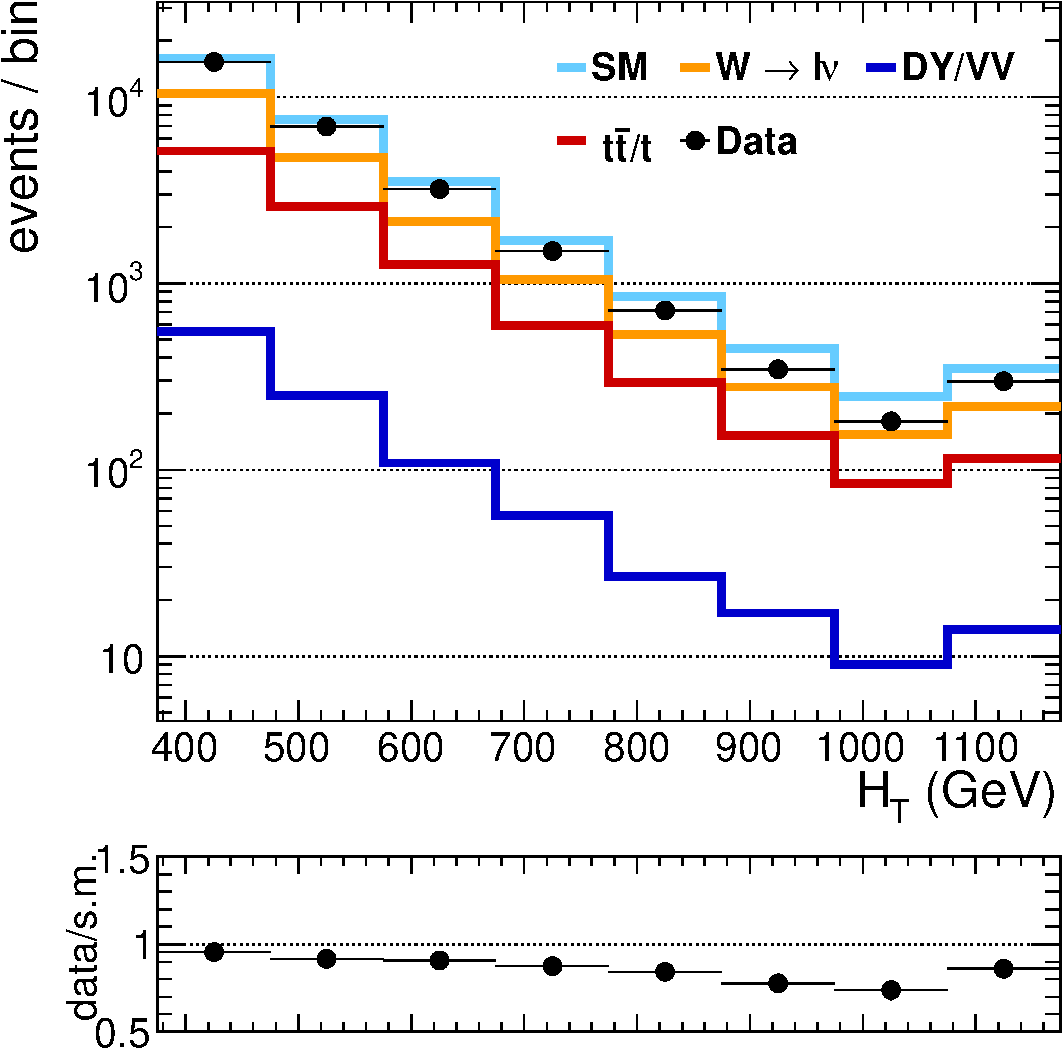
\includegraphics[width=0.4\textwidth,]{figures/data-mc/v22/mu/muonLook_pfJet_ge2j_375_xcak5JetPFSumEtPat.pdf}
  } \\
  \subfigure[\njet distribution (\njethigh, $\nb = 2$)]{
    \label{fig:figures_nj_0}
    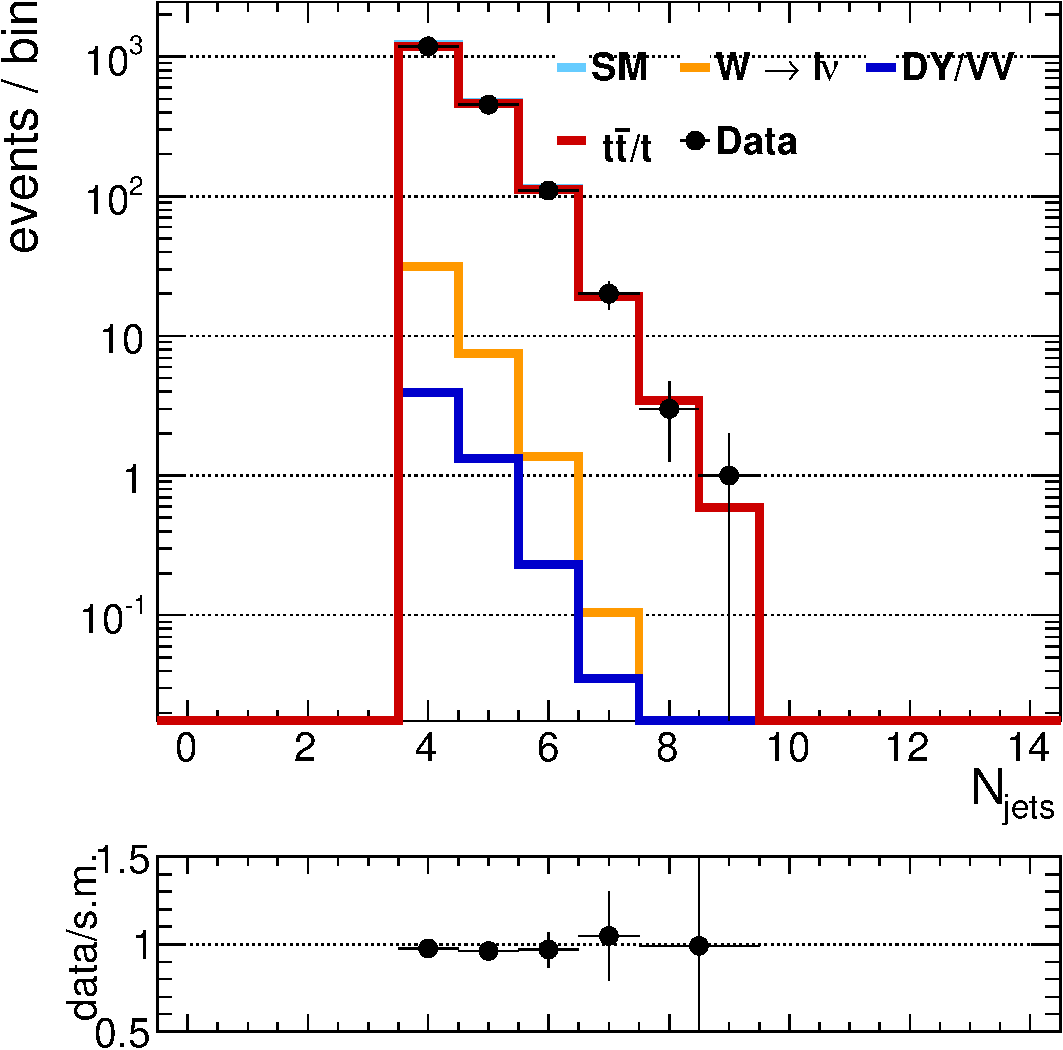
\includegraphics[width=0.4\textwidth,]{figures/data-mc/v22/mu/muonLook_pfJet_ge2j_375_xcak5JetPFIndicesPat_ge4j_eq2b.pdf}
  } 
  \subfigure[\scalht distribution (\njetlow, $\nb = 1$)]{
    \label{fig:figures_HT_1}
    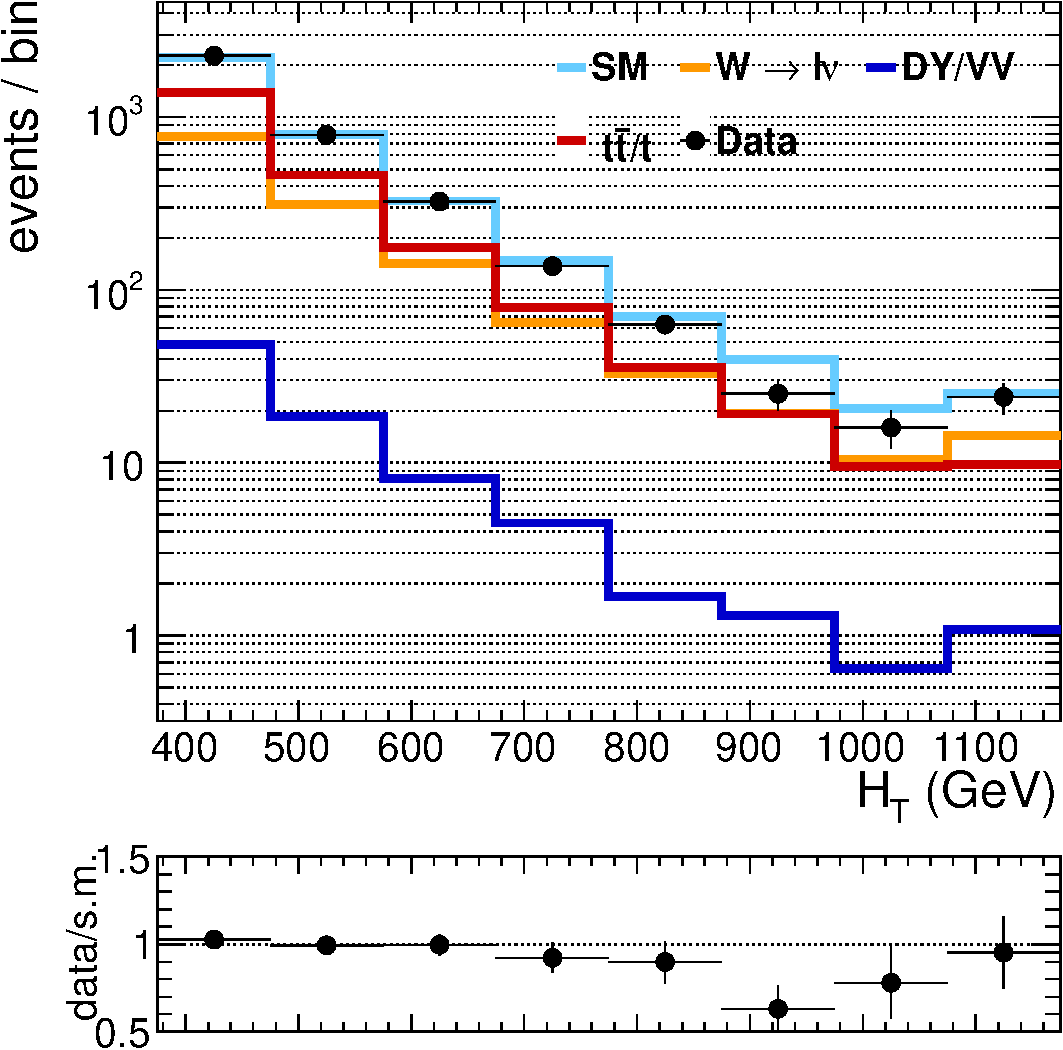
\includegraphics[width=0.4\textwidth,]{figures/data-mc/v22/mu/muonLook_pfJet_ge2j_375_xcak5JetPFSumEtPat_le3j_eq1b.pdf}
  } \\
%\begin{figure}[h!]
%  \centering
%  \subfigure[muon \pt distribution ($\njet \geq 2$, $\nb \geq 0$).]{
%    \label{fig:figures_pt_all}
%    \includegraphics[width=0.4\textwidth,page=163]{figures/data-mc/v22/mu/muonLook_pfJet_ge2j_375.pdf}
%  } 
%  \subfigure[muon $\eta$ distribution ($\njet \geq 2$, $\nb \geq 0$)]{
%    \label{fig:figures_eta_all}
%    \includegraphics[width=0.4\textwidth,page=164]{figures/data-mc/v22/mu/muonLook_pfJet_ge2j_375.pdf}
%  } \\
%  \subfigure[\nb distribution ($\njet \geq 2$, $\nb \geq 0$)]{
%    \label{fig:figures_nb_1}
%    \includegraphics[width=0.4\textwidth,page=187]{figures/data-mc/v22/mu/muonLook_pfJet_ge2j_375.pdf}
%  } 
%  \subfigure[\scalht distribution ($\njet \geq 2$, $\nb \geq 0$)]{
%    \label{fig:figures_HT_0}
%    \includegraphics[width=0.4\textwidth,page=123]{figures/data-mc/v22/mu/muonLook_pfJet_ge2j_375.pdf}
%  } \\
%  \subfigure[\njet distribution (\njethigh, $\nb = 2$)]{
%    \label{fig:figures_nj_0}
%    \includegraphics[width=0.4\textwidth,page=179]{figures/data-mc/v22/mu/muonLook_pfJet_ge2j_375.pdf}
%  } 
%  \subfigure[\scalht distribution (\njetlow, $\nb = 1$)]{
%    \label{fig:figures_HT_1}
%    \includegraphics[width=0.4\textwidth,page=119]{figures/data-mc/v22/mu/muonLook_pfJet_ge2j_375.pdf}
%  } \\
%
  \caption{\label{fig:control-plots-muon} Data--MC comparisons of key
    variables for the muon control region, following the
    application of the full muon control selection selection criteria 
    and the requirements $\scalht > 375\GeV$: (a) muon \pt, (b) muon $\eta$,
    (c) \nb, and (d) \scalht distributions for an inclusive 
    selection on \njet and \nb, and (e) \njet , (f) \scalht distributions for the two 
    event categories (\njethigh, $\nb = 2$) and (\njetlow, $\nb = 1$). }
\end{figure}

\subsubsection{The \texorpdfstring{\gj}{photon plus jets} control sample}

The \znunu + jets background is estimated using \gj events which
have a higher cross-section but similar kinematic properties as 
\znunu + jets when the photon is ignored~\cite{PAS-SUS-08-002,Bern:2011pa}. 
The \gj sample is obtained by requiring exactly one tightly 
identified and isolated photon (as defined in Section~\ref{sec:reconstruction})
with a transverse momentum of at least 165~\gev. The photon is required 
to be contained within the barrel of the detector, ie $|\eta_{\gamma}| <1.44$, 
and to not overlap with any reconstructed jets $\Delta R(\gamma,\textrm{jet}) < 1.0$.
As in the muon control sample, the $\metvec$ is modified to exclude the photon 
when imposing the $\mht/\pfmet<1.25$ selection cut.  All other selections are 
consistent with the hadronic search region including the $\alphat > 0.55$ cut.
Comparisons of data and simulated SM processes key variables relevant to 
the muon control sample are shown in Figure~\ref{fig:control-plots-phot}.

\begin{figure}[h!]
  \centering
  \subfigure[photon \pt distribution ($\njet \geq 2$, $\nb \geq 0$).]{
    \label{fig:figures_pt_all}
    
\includegraphics[width=0.4\textwidth,page=23]{figures/data-mc/v22/phot/photonLook_g_barrel_375_pfJet_ge2j_.pdf}
  } 
  \subfigure[photon $\eta$ distribution ($\njet \geq 2$, $\nb \geq 0$)]{
    \label{fig:figures_eta_all}
    
\includegraphics[width=0.4\textwidth,page=27]{figures/data-mc/v22/phot/photonLook_g_barrel_375_pfJet_ge2j_.pdf}
  } \\
  \subfigure[\alphat distribution ($\njet \geq 2$, $\nb \geq 0$)]{
    \label{fig:figures_at_1}
    
\includegraphics[width=0.4\textwidth,page=47]{figures/data-mc/v22/phot/photonLook_g_barrel_375_pfJet_ge2j_.pdf}
  } 
  \subfigure[\bdphi distribution ($\njet \geq 2$, $\nb \geq 0$)]{
    \label{fig:figures_dphi_0}
    
\includegraphics[width=0.4\textwidth,page=57]{figures/data-mc/v22/phot/photonLook_g_barrel_375_pfJet_ge2j_.pdf}
  } \\
  \subfigure[\scalht distribution (\njetlow, $\nb = 0$)]{
    \label{fig:figures_HT_0}
    
\includegraphics[width=0.4\textwidth,page=90]{figures/data-mc/v22/phot/photonLook_g_barrel_375_pfJet_ge2j_.pdf}
  } 
  \subfigure[\scalht distribution (\njethigh, $\nb = 0$)]{
    \label{fig:figures_HT_1}
    
\includegraphics[width=0.4\textwidth,page=101]{figures/data-mc/v22/phot/photonLook_g_barrel_375_pfJet_ge2j_.pdf}
  } \\
  \caption{\label{fig:control-plots-phot} Data--MC comparisons of key
    variables for the photon control region, following the
    application of the full photon control selection selection criteria 
    and the requirements $\scalht > 375\GeV$: (a) photon \pt, (b) photon $\eta$,
    (c) \nb, and (d) \scalht distributions for an inclusive 
    selection on \njet and \nb, and (e,f) \scalht distributions for the two 
    event categories (\njetlow, $\nb = 0$) and (\njethigh, $\nb = 0$). }
\end{figure}




%\subsection{Increasing the acceptance of the muon control samples\label{sec:larger}}
%
%As described in Sec.~\ref{sec:def-control-samples} above, the
%selection criteria of the three control samples are defined such that
%the background composition and event kinematics of the three control
%samples mirror as closely as possible those for the signal
%region. This is done in order to minimise the reliance on the
%simulation to model correctly the backgrounds and event kinematics in
%the control and signal samples.
%
%However, in the case of the \mj and \mmj samples, no requirement is
%made on \alphat in the selection criteria of the samples. This is made
%possible by the remaining kinematic selection criteria, which are
%sufficiently selective to ensure that the muon samples remain rich in
%events from the \wj, \ttbar and \zmumu processes with negligible
%contamination from QCD multijet events. These selection criteria
%include, for example, requiring exactly one or two tight isolated
%muon(s), and imposing acceptance windows on the invariant mass of the
%di-muon sytem or the transverse mass of the muon-\pfmet system, as
%described above. 

%%The absence of QCD multijet events is demonstrated by the control
%%distributions shown in Sec.~\ref{sec:est-control-samples} below. 
%Thus, the acceptance of the two muon control samples can be
%significantly increased, which simultaneously improves their
%predictive power and further reduces the effect of any potential
%signal contamination.  In the case of the \gj sample (used only for
%the region $\scalht > 375\gev$), the requirement $\alphat > 0.55$ is
%still necessary to suppress contamination from QCD multijet events,
%even after the substantial photon \pt cut in the offline selection.
%
%The extrapolation in the variable \alphat is tested through a
%dedicated set of closure tests, described in Sec.~\ref{sec:bkgd-syst},
%which demonstrate that the different \alphat requirements for the \mj
%and \mmj control samples and signal region have no significant
%systematic bias on the prediction. That the \alphat variable
%introduces no acceptance bias for processes with genuine \met is due
%to the accurate modelling by the CMS simulation of such processes,
%namely W + jets, \ttbar, and \znunu\ + jets. Background estimates for
%these processes are provided by the \mj and \mmj samples, as
%identified at the beginning of this Section. Importantly, the same
%cannot be said for QCD multijet events, as in this case the only
%events that survive the \alphat cut are pathological cases in which a
%jet is severely mismeasured or even lost due to detector
%inefficiencies. Such effects certainly do change the event kinematics
%and, in these cases, an \alphat cut will selectively choose events
%with particular kinematic features and topologies. For these
%pathological cases, one cannot rely on MC to model correctly the
%behaviour and therefore the \alphat acceptance. This is a crucial
%distinction to be made between QCD multijet events and processes with
%significant genuine \met. The assumption is that processes with
%genuine \met are selected by the \alphat variable based on the
%escaping invisible particle(s) rather than any pathological effects.
%
%%\subsection{Distributions from the data control samples\label{sec:est-control-samples}}
%%
%%Distributions of key variables for the \mj, \mmj, and \gj samples are
%%shown in below in Figs.~\ref{fig:mu-distr}, \ref{fig:mumu-distr},
%%and~\ref{fig:phot-distr}, respectively. The first two figures show
%%the (leading) muon \pt and isolation distributions, along with the
%%leading jet \pt, \scalht, \mht and \alphat distributions. For the \gj
%%sample, the photon \pt distribution is%and isolation distributions are
%%shown in place of the corresponding muon distribution.%s.
%%No requirement is made on the number of b-jets per event. In general,
%%the agreement between data and simulation is good, giving confidence
%%that the samples are well understood. The MC distributions highlight
%%the composition of each sample. The contribution from QCD multijet
%%events is expected to be negligible.
%%
%%Figure~\ref{fig:jet-bjet} shows the jet and b-jet multiplicity
%%distributions for the \mj, \mmj, and \gj control samples, as defined
%%in Sec.~\ref{sec:def-control-samples} and following the requirement
%%$\scalht > 375\gev$. An accurate modelling of the jet multiplicity in
%%data is achieved for all samples. The b-jet distributions demonstrate
%%the changing background composition as a function of the number of
%%b-jets. For the \mj and \mmj samples, the requirement of zero b-jets
%%results in sub-samples that are rich in W and Z bosons, respectively,
%%with little contamination from \ttbar. The \ttbar background becomes
%%dominant in the \mj sample when exactly one b-jet is required. The
%%requirement of up to two b-tags per event significantly suppresses all
%%processes except for \ttbar production. Requiring at least three
%%b-tags also suppresses \ttbar production. In the case of the \mmj
%%sample, some contamination from \ttbar is observed for $\nb =
%%1$. Requiring more than one b-jet significantly suppresses the yields
%%in both the \mmj and \gj samples.
%%
%%\clearpage
%%\begin{figure}[!h]
%%  \centering
%%  \subfigure[Muon \pt.]{
%%    \includegraphics[width=0.4\textwidth]{figures/data-mc/v1/muon/Stack_muPt_Muon_all_OneMuon_-1To-2b_log}
%%  } 
%%  \subfigure[Muon isolation.]{
%%    \includegraphics[width=0.4\textwidth]{figures/data-mc/v1/muon/Stack_muonIso_Muon_all_OneMuon_-1To-2b_log}
%%  } \\
%%  \subfigure[Transverse mass.]{
%%    \includegraphics[width=0.4\textwidth]{figures/data-mc/v1/muon/Stack_PFMTmu_Muon_all_OneMuon_-1To-2b_log}
%%  } 
%%  \subfigure[\scalht.]{
%%    \includegraphics[width=0.4\textwidth]{figures/data-mc/v1/muon/Stack_HT_Muon_all_OneMuon_-1To-2b_log}
%%  } \\
%%  \subfigure[\mht.]{
%%    \includegraphics[width=0.4\textwidth]{figures/data-mc/v1/muon/Stack_MHT_Muon_all_OneMuon_-1To-2b_log}
%%  } 
%%  \subfigure[\alphat.]{
%%    \includegraphics[width=0.4\textwidth]{figures/data-mc/v1/muon/Stack_AlphaT_Muon_all_OneMuon_-1To-2b_log}
%%  } 
%%  \caption{Data--MC comparisons of key variables for the \mj control
%%    sample, for the region $\scalht > 275\GeV$. Bands represent the
%%    uncertainties due to the limited size of MC samples. No
%%    requirement on the number of b-jets per event is made.}
%%  \label{fig:mu-distr}
%%\end{figure}
%%
%%\begin{figure}[!h]
%%  \centering
%%  \subfigure[Leading muon \pt.]{
%%    \includegraphics[width=0.4\textwidth]{figures/data-mc/v1/mumu/Stack_muPt_Muon_all_DiMuon_-1To-2b_log}
%%  } 
%%  \subfigure[Muon isolation.]{
%%    \includegraphics[width=0.4\textwidth]{figures/data-mc/v1/mumu/Stack_muonIso_Muon_all_DiMuon_-1To-2b_log}
%%  } \\
%%  \subfigure[Di-muon invariant mass.]{
%%    \includegraphics[width=0.4\textwidth]{figures/data-mc/v1/mumu/Stack_Zmass_Muon_all_DiMuon_-1To-2b_log}
%%  } 
%%  \subfigure[\scalht.]{
%%    \includegraphics[width=0.4\textwidth]{figures/data-mc/v1/mumu/Stack_HT_Muon_all_DiMuon_-1To-2b_log}
%%  } \\
%%  \subfigure[\mht.]{
%%    \includegraphics[width=0.4\textwidth]{figures/data-mc/v1/mumu/Stack_MHT_Muon_all_DiMuon_-1To-2b_log}
%%  } 
%%  \subfigure[\alphat.]{
%%    \includegraphics[width=0.4\textwidth]{figures/data-mc/v1/mumu/Stack_AlphaT_Muon_all_DiMuon_-1To-2b_log}
%%  } 
%%  \caption{Data--MC comparisons of key variables for the \mmj control
%%    sample, for the region $\scalht > 275\GeV$. Bands represent the
%%    uncertainties due to the limited size of MC samples. No
%%    requirement on the number of b-jets per event is made.}
%%  \label{fig:mumu-distr}
%%\end{figure}
%%
%%\begin{figure}[!h]
%%  \centering
%%  \subfigure[Photon \pt.]{
%%    \includegraphics[width=0.4\textwidth]{figures/data-mc/v1/photon/Stacked_PhotonPt_all_Photon_375_upwards}
%%  } 
%%  \subfigure[\scalht.]{
%%    \includegraphics[width=0.4\textwidth]{figures/data-mc/v1/photon/Stacked_HT_after_alphaT_55_all_Photon_375_upwards}
%%  } \\
%%  \subfigure[\mht.]{
%%    \includegraphics[width=0.4\textwidth]{figures/data-mc/v1/photon/Stacked_MHT_after_alphaT_55_all_Photon_375_upwards}
%%  } 
%%  \subfigure[\alphat.]{
%%    \includegraphics[width=0.4\textwidth]{figures/data-mc/v1/photon/Stacked_AlphaT_all_Photon_375_upwards}
%%  } 
%%  \caption{Data--MC comparisons of key variables for the \gj control
%%    sample, for the region $\scalht > 375\GeV$. Bands represent the
%%    uncertainties due to the limited size of MC samples. No
%%    requirement on the number of b-jets per event is made.}
%%  \label{fig:phot-distr}
%%\end{figure}
%%
%%\begin{figure}[!h]
%%  \centering
%%  \subfigure[\njet for the \mj sample.]{
%%    \includegraphics[width=0.4\textwidth]{figures/data-mc/v1/muon/Stack_ncommjet_Muon_all_OneMuon_-1To-2b_log}
%%  } 
%%  \subfigure[\njet for the \mmj sample.]{
%%    \includegraphics[width=0.4\textwidth]{figures/data-mc/v1/mumu/Stack_ncommjet_Muon_all_DiMuon_-1To-2b_log}
%%  } \\
%%  \subfigure[\njet for the \gj sample.]{
%%    \includegraphics[width=0.4\textwidth]{figures/data-mc/v1/photon/Stacked_JetMultiplicityAfterAlphaT_55_all_Photon_375_upwards}
%%  } 
%%  \subfigure[\nb for the \mj sample.]{
%%    \includegraphics[width=0.4\textwidth]{figures/data-mc/v1/muon/Stack_nbjet_Muon_all_OneMuon_-1To-2b_log}
%%  } \\
%%  \subfigure[\nb for the \mmj sample.]{
%%    \includegraphics[width=0.4\textwidth]{figures/data-mc/v1/mumu/Stack_nbjet_Muon_all_DiMuon_-1To-2b_log}
%%  } 
%%  \subfigure[\nb for the \gj sample.]{
%%    \includegraphics[width=0.4\textwidth]{figures/data-mc/v1/photon/Stacked_Btag_Post_AlphaT_5_55_all_Photon_375_upwards}
%%  } 
%%  \caption{Data--MC comparison of the number of reconstructed jets
%%    (top) and b-jets (bottom) per event in the (left) \mj sample,
%%    (middle) \mmj sample, and (right) \gj control sample. Bands
%%    represent the uncertainties due to the limited size of MC
%%    samples.}\label{fig:jet-bjet}
%%\end{figure}
%
%%\subsection{Translation factors and ``na\"ive'' predictions\label{sec:est-control-samples}}
%%
%%Appendix~\ref{app:tf} contains tables summarising the observed and
%%expected yields from data and simulation, in, respectively the bins of
%%the three control samples. Also listed are the expectations from
%%simulation for the various background contributions in the signal
%%region, along with the corresponding translation factors. The yields
%%are binned in \scalht, jet multiplicity and number of b-jets per
%%event. The errors associated with the translation factors reflect the
%%uncertainty due to the finite size of the MC samples used to determine
%%the factors. Any trigger inefficiency is also factored into the
%%translation factors (\ie, the trigger is effectively emulated and
%%yields from the MC samples are corrected to account for any
%%inefficiency). Also, all MC expectations are corrected to account for
%%any discrepancies between data and MC for the efficiency and mistag
%%rate of the b-tagging algorithm used, as described further in
%%Sec.~\ref{sec:btag-eff-correction}. However, no systematic
%%uncertainties on the translation factors are quoted in the tables.
%%
%%The same tables also list ``na\"ive'' predicted yields obtained from
%%each control sample for individual SM backgrounds in the signal region
%%(\eg, W + jets and \ttbar from the \mj sample, and \znunu + jets from
%%the \mmj and \gj samples). These predictions are given for
%%illustrative purposes only. For the analysis result, the predictions
%%for the total SM background are determined by a fit to the yields in
%%the signal region and all three control samples, as described in
%%Sec.~\ref{sec:statistics}. In addition to observed yields, the fit
%%takes as input the translation factors with their associated
%%statistical and systematic uncertainties. 
%%
%%Illustrative predictions for the total SM background can be made for
%%each bin in the signal region, by combining the individual
%%predictions. One such combination can be made by using the individual
%%predictions from the \mj and \mmj samples (or, alternatively, the
%%predictions from the \mj and \gj samples), the result of which can be
%%compared with the observed yields in the bins of the signal
%%region. Predictions in this way are made for bins of the three
%%exclusive b-tag categories requiring exactly zero and one b-tags per
%%event. When requiring at least two b-tagged jets per event, only the
%%\mj sample has sufficiently large yields to predict accurately the
%%total SM background. The errors on the total SM predictions reflect
%%statistical uncertainties only. It is again noted that these
%%``na\"ive'' predictions are for illustration only, with the final SM
%%expectations for all signal region bins given by the simultaneous fit
%%to yields in all data samples. Table~\ref{tab:tf-summary} summarises
%%the contents of the various sections in the Appendix that list tables
%%containing observed yields, MC expectations, translation factors, and
%%``na\"ive'' predictions for individual and total SM backgrounds.
%%
%%\begin{table}[h!]
%%  \caption{Each section in Appendix~\ref{app:tf} contains tables that
%%    list: observed yields, MC expectations, translation factors, and
%%    ``na\"ive'' predictions for individual SM backgrounds, for each of
%%    the \mj, \mmj, and \gj control samples; and total SM predictions
%%    when combining the individual predictions from the \mj and \mmj
%%    samples and the \mj and \gj samples, separately.}
%%  \label{tab:tf-summary}
%%  \centering
%%  \footnotesize
%%  \begin{tabular}{ llll }
%%    \hline
%%    Section            & \njet bin & \nb bin & Control samples used \\ [0.5ex]
%%    \hline
%%    \ref{app:23j0b}    & 2--3      & 0       & \mj, \mmj, \gj       \\
%%    \ref{app:23j1b}    & 2--3      & 1       & \mj, \mmj, \gj       \\
%%    \ref{app:23j2b1mu} & 2--3      & 2       & \mj                  \\
%%    \ref{app:4j0b}     & $\geq$4   & 0       & \mj, \mmj, \gj       \\
%%    \ref{app:4j1b}     & $\geq$4   & 1       & \mj, \mmj, \gj       \\
%%    \ref{app:4j2b1mu}  & $\geq$4   & 2       & \mj                  \\
%%    \ref{app:4j3b1mu}  & $\geq$4   & 3       & \mj                  \\
%%    \ref{app:4j4b1mu}  & $\geq$4   & $\geq$4 & \mj                  \\
%%    \hline
%%  \end{tabular}
%%\end{table}
%
%
%%\begin{table}[h!]
%%  \caption{}
%%  \label{tab:}
%%  \centering
%%  \footnotesize
%%  \begin{tabular}{ lll }
%%    \hline
%%    \hline
%%    \njet bin & \nb bin & Control samples used \\ [0.5ex]
%%    \hline
%%    2--3      & 0       & \mj, \mmj, \gj       \\
%%    2--3      & 1       & \mj, \mmj, \gj       \\
%%    2--3      & 2       & \mj                  \\
%%    $\geq$4   & 0       & \mj, \mmj, \gj       \\
%%    $\geq$4   & 1       & \mj, \mmj, \gj       \\
%%    $\geq$4   & 2       & \mj                  \\
%%    $\geq$4   & 3       & \mj                  \\
%%    $\geq$4   & $\geq$4 & \mj                  \\
%%    \hline
%%    \hline
%%  \end{tabular}
%%\end{table}

